% ------------------------------------------------------------------------------
%
% PREAMBLE
%
% ------------------------------------------------------------------------------

\documentclass[12pt, titlepage]{article}


\usepackage{graphicx, amsmath, amssymb, natbib, setspace, sectsty, verbatim, 
		mathrsfs, float}
\usepackage{MnSymbol}
\usepackage{multirow}
\usepackage{bm}
\usepackage[usenames, dvipsnames]{color}
\bibpunct{(}{)}{;}{a}{}{,}
\setlength{\parindent}{3em}
%\parskip = 1.5ex
%\linespread{1.3}
%\onehalfspacing

\pdfpagewidth 8.5in
\pdfpageheight 11in
\setlength{\oddsidemargin}{0.0in} \setlength{\textwidth}{6.5in}
\setlength{\topmargin}{0.15in} \setlength{\textheight}{8.5in}
\setlength{\headheight}{0.0in} \setlength{\headsep}{0.0in}

\usepackage{/mnt/ExtraDrive1/Work/shTex/mymacros}

\providecommand{\norm}[1]{\lVert#1\rVert}
\newcommand{\csection}[1]{\section[#1]{\centering #1 }}
\subsectionfont{\small}
\newcommand{\cye}[1]{\color{yellow!70!black}#1}
\newcommand{\cre}[1]{\color{red!70!black}#1}
\newcommand{\cbl}[1]{\color{blue!70!black}#1}
\newcommand{\cgr}[1]{\color{green!70!black}#1}


% ------------------------------------------------------------------------------
%
% BEGIN DOCUMENT
%
% ------------------------------------------------------------------------------

\begin{document}

\setcounter{equation}{0}
\renewcommand{\theequation}{R.\arabic{equation}}


% ------------------------------------------------------------------------------
%
%                    Section 8.8.3
%                    The wet sulfate desposition data
%
% ------------------------------------------------------------------------------

{\large \flushleft \textbf{8.8.3 The wet sulfate desposition data}}

\vspace{.3cm}

Exploratory data analysis scattered throughout Chapter 3 suggested that it would be wise to transform the wet sulfate deposition data to the square-root scale and to set aside three outliers, yielding a modified dataset that was called the clean wet sulfate deposition data.  Polynomials of orders zero through five were fitted to these modified data by OLS in Section 4.5.3, and summary statistics from these fits suggested that polynomials up to third-order (and possibly higher) were worthy of further consideration.  The analyses presented in Section 4.5.3 also suggested that spatial autocorrelation exists and is isotropic in the residuals from the quadratic fit, but perhaps does not exist in the residuals from the cubic and higher-order fits.

\begin{figure}[H]
  \begin{center}
	    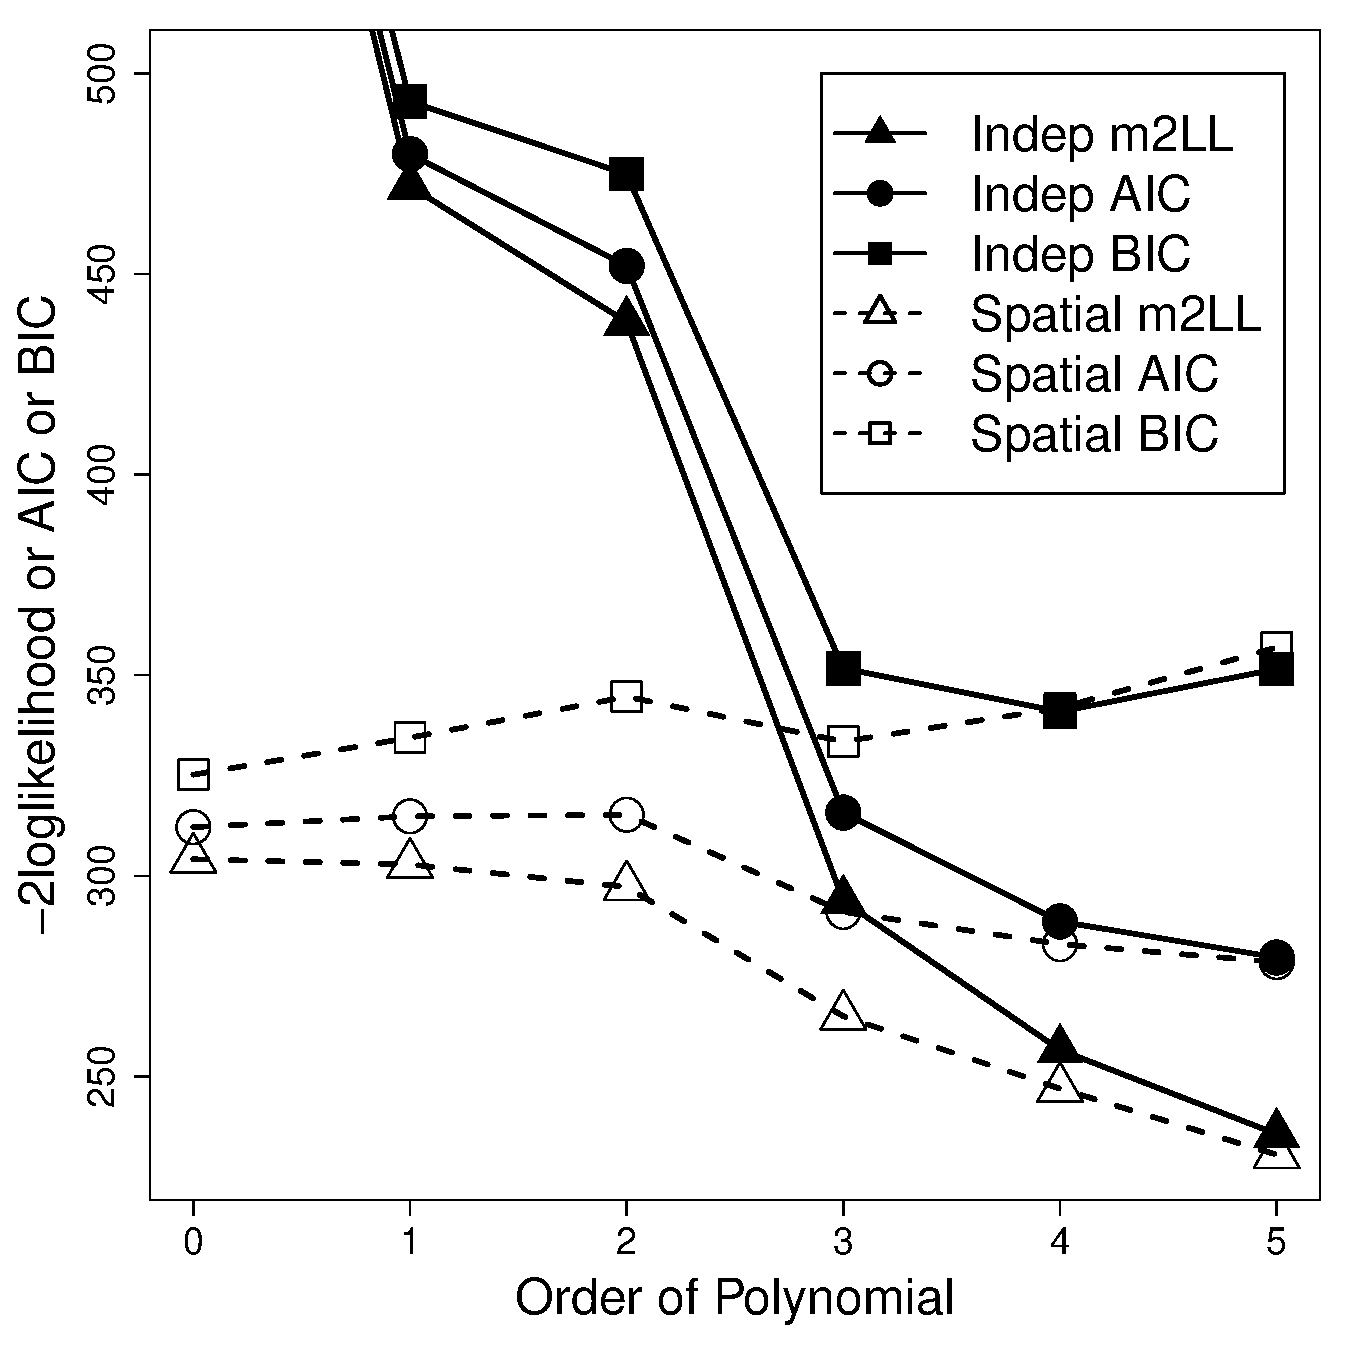
\includegraphics[width=.6\linewidth]{SO4_AIC}
  \end{center}
  \caption{Two times the negative log-likelihood (m2LL, triangles), AIC (circles), and BIC (squares) for polynomial models on the spatial coordinates, for both independent error models (solid lines and solid shapes) and spatial models (dashed line and open shapes). \label{Fig:SO4_AIC}}
\end{figure}

Here, we fit polynomial models to the clean wet sulfate deposition data once again, but this time using likelihood-based methods.  Models having polynomial mean structures up to (and including) order five and having several geostatistical covariance functions were estimated by MLE using the \texttt{R} package \texttt{spmodel}, which also returns AIC and the log-likelihood, from which we computed BIC.  Figure~\ref{Fig:SO4_AIC} shows $-2\log\l(\bar{\boldsymbol{\beta}},\bar{\boldsymbol{\theta}})$ (which we denote as m2LL), AIC, and BIC computed for all polynomial models on the two spatial coordinates from the constant mean model up to a fifth-order polynomial for both independent error models and spatially-autocorrelated error models, where the spatial autocorrelation is an exponential model. Note that m2LL decreases as the order of the polynomial increases, as it must, because the models are nested. AIC and BIC are greater than m2LL due to their respective penalties that depend on the number of parameters and sample size, which is readily seen in Figure~\ref{Fig:SO4_AIC}. 
\begin{figure}[H]
  \begin{center}
	    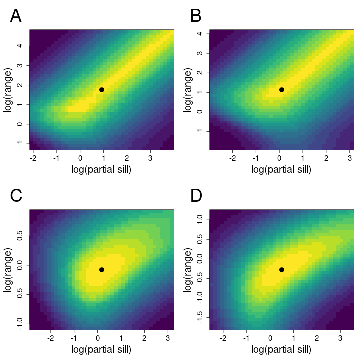
\includegraphics[width=.8\linewidth]{SO4_Viz_m2LL_covParms}
  \end{center}
  \caption{Surface of the restricted log-likelihood for the logarithm of the partial sill ($\log(\theta_{1})$) by the logarithm of the range parameters ($\log(\theta_{2})$ while holding the nugget effect constant at its restricted maximum likelihood estimate. A. Circular model. B. spherical model. C. Gaussian model. D. Gravity model.  The more yellow colors are larger likelihood values, and the bluer colors are smaller likelihood values. The REML estimates are shown as solid black circles. \label{Fig:SO4_psill_range}}
\end{figure} 
For both the independent models and spatial models, AIC generally decreases most rapidly between the 2nd and 3rd orders of the polynomials, and continues to decrease, but more slowly for higher order polynomials. AIC has a reputation for favoring overly complex models, so we also show BIC (Figure~\ref{Fig:SO4_AIC}).  While AIC suggests that the ``best'' model is a 5th order polynomial for both independence and spatial models, BIC suggests that a 4th order polynomial is best if assuming the errors are independent, while BIC suggests that a constant mean model is best when considering spatially autocorrelated models.  We will consider model selection for these data in more detail after we introduce prediction in Chapter 9.

Fitting spatial models is more complicated than fitting models where errors are assumed independent.  One feature of almost all models listed in Table 6.1 is that there is ``correlation'' in the likelihood between $\theta_{1}$, the partial sill, and $\theta_{2}$, the range parameter.  To investigate this, we use REMLE for a constant mean model for the circular, spherical, Gaussian, and gravity models, Figure~\ref{Fig:SO4_psill_range}), which plots the log-likelihood as a function of the logarithms of the range ($\theta_{2}$) and partial sill ($\theta_{1}$) parameters.

In fact, \citet{zhang_inconsistent_2004} shows that estimation of $\theta_{1}$ and $\theta_{2}$ are asymptotically inconsistent, but estimation of their ratio $\theta_{1}/\theta_{2}$ is asymptotically consistent.  This is most apparent in the long ridge in Figure~\ref{Fig:SO4_psill_range}B. There are nearly equal likelihood values all along this ridge, and, in fact, practitioners of geostatistics are well aware that sometimes optimization does not converge as both the range and partial sill increase along this ridge. However, \citet{zhang_inconsistent_2004} also shows that predictions and their standard errors are largely insensitive to the values of $\theta_{1}$ and $\theta_{2}$ themselves, but are sensitive to their ratio.  Thus, it matters little where estimates settle on the ridge seen in Figure~\ref{Fig:SO4_psill_range}B because the ratio remains relatively constant.  Practitioners of geostatistics have also been aware of this for years, and often set a bound on one of these parameters to force convergence, realizing that little changes by letting the range and partial sill continue to increase during optimization.

It is also instructive to look at the likelihood by allowing the partial sill and nugget to vary, while holding the range parameter constant.  The resulting surface for the spherical model shown in Figure~\ref{Fig:SO4_psill_range}B is given in Figure~\ref{Fig:SO4_psill_nugget}. Notice that there is negative correlation between the partial sill and nugget in the likelihood.  This makes sense because there is only so much variation in the data. If we think of the total variance as (nugget + partial sill), then if one goes up, the other must go down, and that is expressed in the likelihood shown in Figure~\ref{Fig:SO4_psill_nugget}.
\begin{figure}[H]
  \begin{center}
	    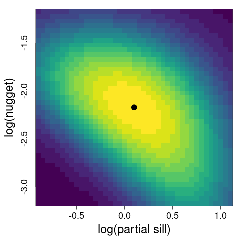
\includegraphics[width=.5\linewidth]{SO4_psillvsnugget}
  \end{center}
  \caption{Likelihood surface for the logarithm of the partial sill, $\log(\theta_{1})$, by the logarithm of the nugget parameter, $\log(\theta_{0})$, while holding the range parameter constant at its restricted maximum likelihood estimate. The REML estimate is shown as a solid black circle. \label{Fig:SO4_psill_nugget}}
\end{figure}

The curvature of the likelihood at the REMLE (or MLE) is approximated by Fisher's Information matrix, which can be used to construct confidence intervals as suggested earlier.  After fitting the model, we can easily compute 
$$
\boldsymbol{F}_{a}{(\boldsymbol{\theta})_{i,j}} = \frac{1}{2}\operatorname{tr}\left(\boldsymbol{\Sigma}^{-1} \frac{\partial \boldsymbol{\Sigma}}{\partial\theta_i}{\boldsymbol{\Sigma}^{-1}}\frac{\partial\boldsymbol{\Sigma}}{\partial\theta_j}\right),
$$
by noting the general form $\boldsymbol{\Sigma} = \theta_{1}\mathbf{R}(\theta_{2}) + \theta_{0}\mathbf{I}$, and hence $\partial \boldsymbol{\Sigma}/ \partial \theta_0 = \mathbf{I}$, $\partial \boldsymbol{\Sigma}/ \partial \theta_1 = \mathbf{R}(\theta_{2})$ and $\partial \boldsymbol{\Sigma}/ \partial \theta_2 = \theta_{1}\mathbf{A}$, where $\mathbf{A}$ is a matrix constructed based on the estimated parameters and distance in $\partial \sigma(r,\boldsymbol{\theta})/\partial \theta_{2}$ (Table 6.1).  For example, if $\mathbf{D}$ is the matrix of all pairwise distances, and we chose an exponential model, then $\mathbf{A} = \mathbf{D}\odot\mathbf{R}/\theta_{2}^{2}$, where $\odot$ is the Hadamard or direct product.  Then the asymptotic standard errors are the square roots of the diagonal of $\boldsymbol{F}^{-1}_{a}{(\boldsymbol{\theta})}$.  We fitted constant mean models with REMLE, and the estimated values of covariance parameters for various autocovariance models, along with their estimated standard errors based on Fisher's Information, are given in Table~\ref{tab:AsySE}.

Another approach is to compute the Hessian matrix of the log-likelihood.  We used \texttt{spmodel} for this as it allowed us to evaluate the log-likelihood for any given value of $\boldsymbol{\theta}$.  We used the \texttt{R} package \texttt{numDeriv} to compute the numeric Hessian, $\mathbf{H}$, at the REMLE, and then an estimator of Fisher's Information is,
$$
\boldsymbol{F}_{n}{(\boldsymbol{\theta})} = -\mathbf{H},
$$
and an estimator of the asymptotic standard errors are the square roots of the diagonal of $\boldsymbol{F}^{-1}_{n}{(\boldsymbol{\theta})}$.  The estimated standard errors for each covariance parameter based on this numeric Hessian for a variety of models are given in Table~\ref{tab:AsySE}, which can be compared to the analytic counterpart.

\begin{table}[H] 
				\caption{Estimated covariance parameters using REML, and estimated standard errors of those covariance parameters using the analytical solution to Fisher's Information, and estimated standard errors using am estimator of Fisher's Information based a numeric Hessian.\label{tab:AsySE}}
\begin{center}
\begin{tabular}{|c|rrr|rrr|rrr|}
  \hline
  \hline{}
  & \multicolumn{3}{c|}{Estimate} & \multicolumn{3}{c|}{Analytic SE} & \multicolumn{3}{c|}{Numeric SE}\\
  Model & psill & nugget & range & psill & nugget & range & psill & nugget & range \\
	\hline
  \hline
exponent & 2.653 & 0.111 & 4.598 & 2.374 & 0.026 & 4.322 & 3.919 & 0.023 & 6.958 \\ 
  spherical & 1.091 & 0.115 & 3.085 & 0.133 & 0.038 & 0.450 & 0.254 & 0.023 & 0.205 \\ 
  gaussian & 1.197 & 0.190 & 0.920 & 0.328 & 0.054 & 0.220 & 0.458 & 0.023 & 0.119 \\ 
  gravity & 1.624 & 0.170 & 0.761 & 0.733 & 0.021 & 0.159 & 0.719 & 0.022 & 0.161 \\ 
  rquad & 1.285 & 0.173 & 0.960 & 0.547 & 0.021 & 0.172 & 0.523 & 0.022 & 0.180 \\ 
  magnetic & 1.205 & 0.175 & 1.140 & 0.500 & 0.021 & 0.187 & 0.475 & 0.022 & 0.203 \\ 
  circular & 2.405 & 0.113 & 5.453 & 1.631 & 0.026 & 3.656 & 1.625 & 0.023 & 3.438 \\ 
  \hline
  \hline
\end{tabular}
\end{center}
\end{table}

Besides the diagonal elements of the asymptotic covariance matrix of $\boldsymbol{\theta}$, it is interesting to look at the correlation among the parameters, which, for the circular model in Table~\ref{tab:AsySE}, and the parameter order is partial sill, nugget, range, is 
$$
\left(
\begin{array}{ccc}
1.0000 & -0.1341 & 0.9326 \\ 
  -0.1341 & 1.0000 & 0.0979 \\ 
  0.9326 & 0.0979 & 1.0000 \\ 
\end{array}
\right).
$$
Here, as in Figure~\ref{Fig:SO4_psill_range}A, we can see the strong correlation between the partial sill and the range, and, as in Figure~\ref{Fig:SO4_psill_nugget}, the weaker, but still evident, negative correlation between the partial sill and the nugget.
  
In Figures~\ref{Fig:SO4_psill_range} and \ref{Fig:SO4_psill_nugget} it has been useful to examine the likelihood surface by plotting two parameters at a time to look for multi-modality and unusual interactions, and the construction of the asymptotic covariance matrix of the covariance parameters reveals the same features and can be used to construct confidence intervals.  Another way to assess covariance parameter estimation is to use profile likelihood.  Consider the REML function $L_{-i,R}(\theta_{i};\hat{\boldsymbol{\theta}}_{-i},\hat{\boldsymbol{\beta}},\mathbf{y})$, where the $i$th component of $\boldsymbol{\theta}$ has been held constant at $\theta_{i}$, and the function has been maximized for all other parameters, whose values are denoted as $\hat{\boldsymbol{\theta}}_{-i}$ and $\hat{\boldsymbol{\beta}}$.  Note that $\hat{\boldsymbol{\theta}}_{-i}$ and $\hat{\boldsymbol{\beta}}$ change with each $i$, but we suppress any notation to indicate such dependence. Then a profile likelihood plot for the $i$th component of $\boldsymbol{\theta}$ is one which plots $L_{-i,R}(\theta_{i};\hat{\boldsymbol{\theta}}_{-i},\hat{\boldsymbol{\beta}},\mathbf{y})$ for various values of $\theta_{i}$. 
\begin{figure}[H]
  \begin{center}
	    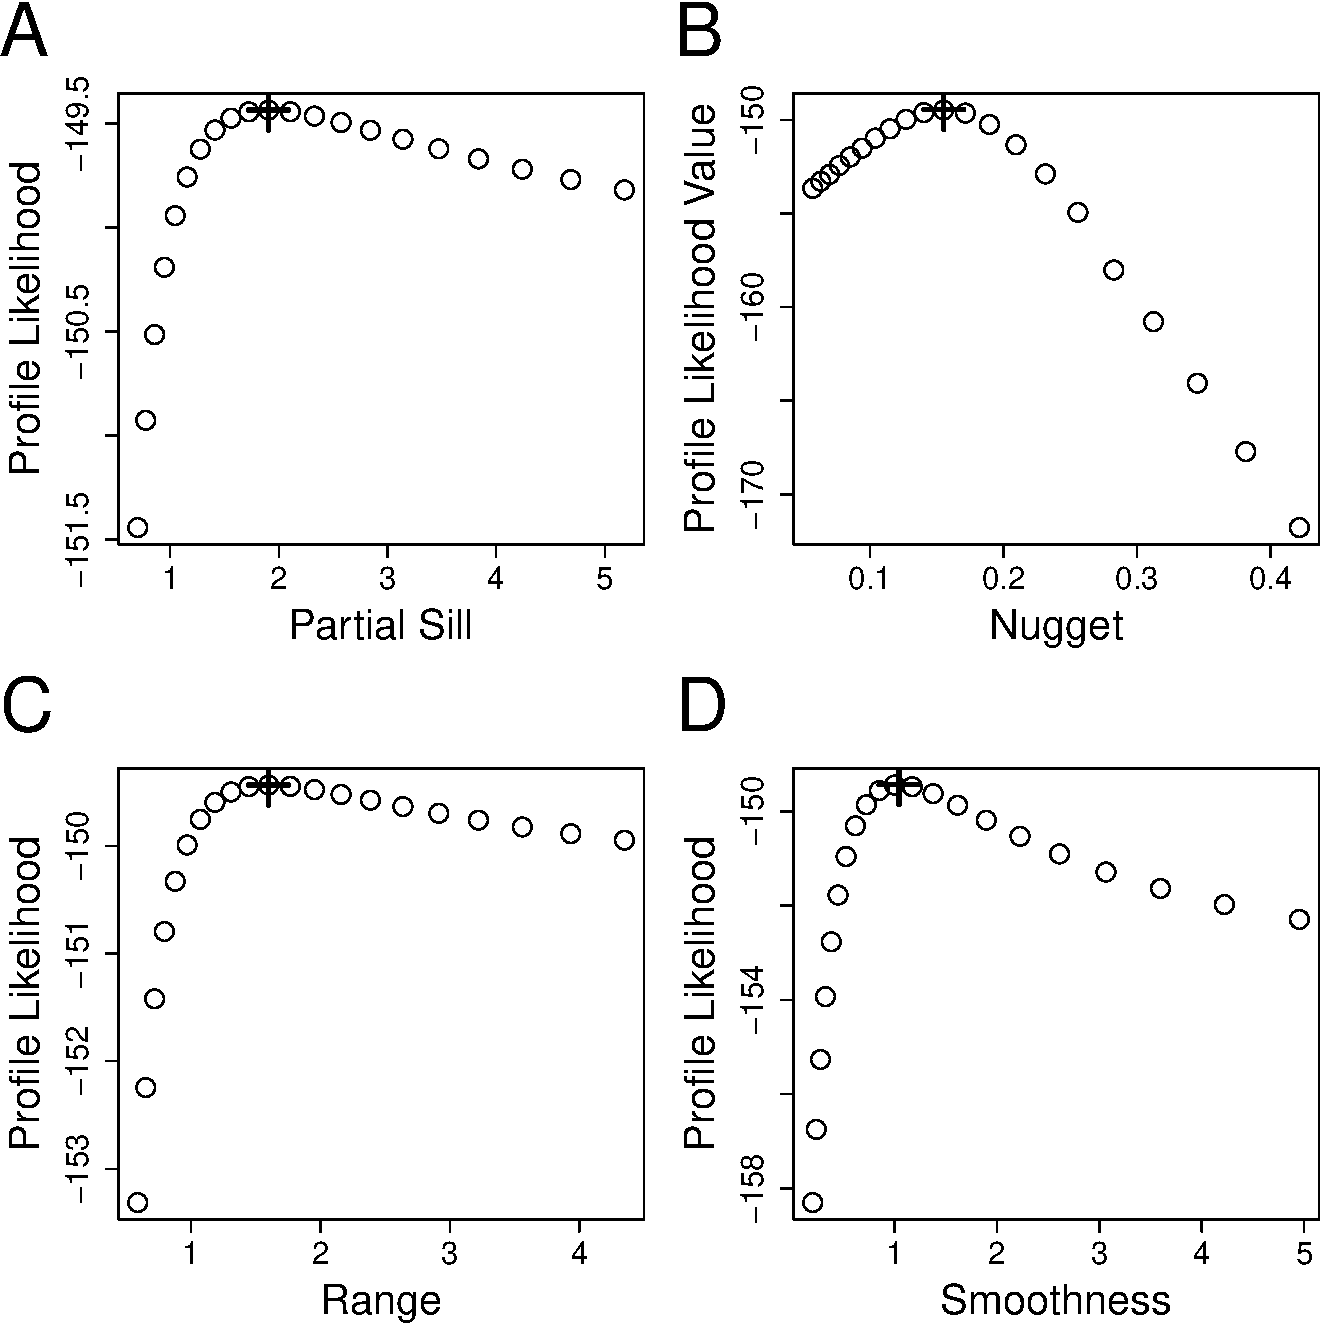
\includegraphics[width=.8\linewidth]{Matern_SO4}
  \end{center}
  \caption{Profile likehood for parameters in Matern model fitted to SO4 data with a constant mean. A. Partial Sill, B. Nugget, C. Range, and D. Smoothness.  For each parameter, the REML estimate is shown by a + and the value of the log likelihood at the REML estimate. \label{Fig:Matern_SO4}}
\end{figure}


Let us consider the Matern covariance function, which is very popular because it has an additional parameter that controls smoothness and differentiability of the surface that it produces.  In Table 6.1, this is denoted at $\theta_{3}$, and we will call it the smoothness parameter. If $\theta_{3} = 1/2$, then the Matern model is equivalent to the exponential model, if $\theta_{3} = 1$ is has been called the Whittle model, if $\theta_{3} = 3/2$ it is a radon model of order 2, if $\theta_{3} = 5/2$ it is a radon model of order 4, and as $\theta_{3} \rightarrow \infty$, the Matern model is equivalent to a Gaussian model.  In \texttt{spmodel}, the smoothness parameter is allowed to range from $1/5$ to 5.  For the Matern model, Figure~\ref{Fig:Matern_SO4}  shows the profile likelihood decreasing slowly as values for the partial sill and range increase beyond their REMLEs.  The nugget has a pronounced peak in the profile likelihood.  Some authors claim that the smoothness parameter for the Matern model is difficult to estimate, and they suggest either picking a single value, or pick several, and choose one based on the likelihood or other model selection criteria.  However, for these data, the smoothness parameter has a fairly well-defined maximum, and optimization had no issues.


%%%%%%%%%%%%%%%%%%%%%%%%%%%%%%%%%%%%%%%%%%%%%%%%%%%%%%%%%%%%%%%%%%%%%%%%%%%%%%%%%%
%%%%%%%%%%%%%%%%%%%%%%%%%%%%%%%%%%%%%%%%%%%%%%%%%%%%%%%%%%%%%%%%%%%%%%%%%%%%%%%%%%
%                BIBLIOGRAPHY
%%%%%%%%%%%%%%%%%%%%%%%%%%%%%%%%%%%%%%%%%%%%%%%%%%%%%%%%%%%%%%%%%%%%%%%%%%%%%%%%%%
%%%%%%%%%%%%%%%%%%%%%%%%%%%%%%%%%%%%%%%%%%%%%%%%%%%%%%%%%%%%%%%%%%%%%%%%%%%%%%%%%%

%\bibliographystyle{consbiol}
\bibliographystyle{/mnt/ExtraDrive1/Work/shTex/asa}
\bibliography{DaleChap883.bib}
%\bibliographystyle{/home/jay/Data/shTex/shTex/asa}
%\bibliography{/home/jay/Data/shTex/shTex/StatBibTex.bib}

\end{document}

